% úvod
Zde bych rád rozebral jak budu jednotlivé požadavky řešit. Nastínil jak bude celkové řešení vypadat, strukturu\ldots Též 
bych zde rád představil kde vlastně budu měřit a zpracovávat data.

% měření
Ohledně měření bych zatím zmínil jen frekvence o které myslím myslím, že pro mé účely bude stačit měřit jednou za čtvrt 
hodiny, to je 96 měření za den. Neodchytím tím sice drobné výkyvy v rámci minut, ale cílem je zachytit dlouhodobý průběh 
hodnot v rámci dne, kdy mne tak drobné výkyvy nezajímají. Pro tento účel by se čtvrt hodiny mohlo zdát možná až jako 
příliš často, ale já bych to tak nechal z důvodu zjemnění denních grafů, přeci jenom graf se třeba 12 hodnotami nevypadá 
úplně nejlépe, a také z důvodu odchycení případných chyb měření nebo náhlých změn, například při zalévání atd.

% ukládání
Co se týče uložení dat, abych zajistil stoprocentní jistotu, že se data uloží, budu je ukládat přímo v místě měření, tím 
myslím, že počítač, který bude mít na starosti měřit, bude zároveň naměřená data hned ukládat na SD kartu, nebo tak 
někam. Bude to takový log měření, který mi umožní obnovit data nezapsaná do cloudu z důvodu nějaké chyby, případně mi 
umožní zjišťovat kde vlastně chyba nastala, a může pomoci i s řešením. Dále myslím, že data bude stačit ukládat klidně 
pouze na jedno místo v cloudu, poněvadž ten sám o sobě pokud je kvalitní je výborně zálohovaný, pokud o data v něm 
nějakým nedopatřením přijdu, nějak mě to neovlivní, bude to škoda, avšak závažné důsledky to mít nebude a navíc tím, že 
nebudu řešit zálohy a rozkopírovávání dat, či jejich konzistenci na různých místech se celé řešení výrazně zjednoduší.

% data flow
Teď se dostávám k samotnému data flow, tedy jak a kam mi potečou data co naměřím. Začnu u senzoru, ten změří data 
a pošle je do obslužného počítače, to může být v podstatě cokoli se schopností ovládat senzor,ukládat data a schopností 
poslat data přes wifi. Ten data zaloguje na perzistentní úložiště a pošle je na centrální bránu pomocí wifi sítě, což mi 
přijde nejednoduší, nemusím nikde tahat kabely, či řešit jiné bezdrátové technologie, poněvadž wifi síť má v místě 
měření dostatečné pokrytí. Teď se dostávám k takovému kontroverznímu prvku celého flow, a tím je centrální brána. To je 
v podstatě počítač, který jediný co dělá je přeposílání dat ze senzorů někam jinam, dal by se tedy úplně odstranit s tím 
že měřící stanice by data odesílala přímo do internetu, ale já ji zahrnul z těchto důvodů. Díky tomu, že s internetem 
komunikuje pouze jedna stanice nemusím na ostatních řešit jejich autentizaci vůči cloudu, či různé SSL certifikáty 
a podobně. To mi umožní na jejich místech mohu nasadit mnohem jednoduší zařízení. Dále mi to umožní přístup k datům doma 
i bez internetu, kdybych si je chtěl nějak zobrazit... A Také to zjednoduší ladění celého systému, kdy například 
programy mohu testovat u sebe na počítači kdy data budu brát z centrální brány a nebudu muset vůbec zasahovat do kódu 
v senzoru. No a to je celé z brány pošlu data do cloudu a tam jejich cesta končí, pokud tedy vynechám cestu z cloudu za 
účelem jejich zobrazení.
\begin{figure}[h]
		\caption{Takto přibližně potečou data}
		\centering
		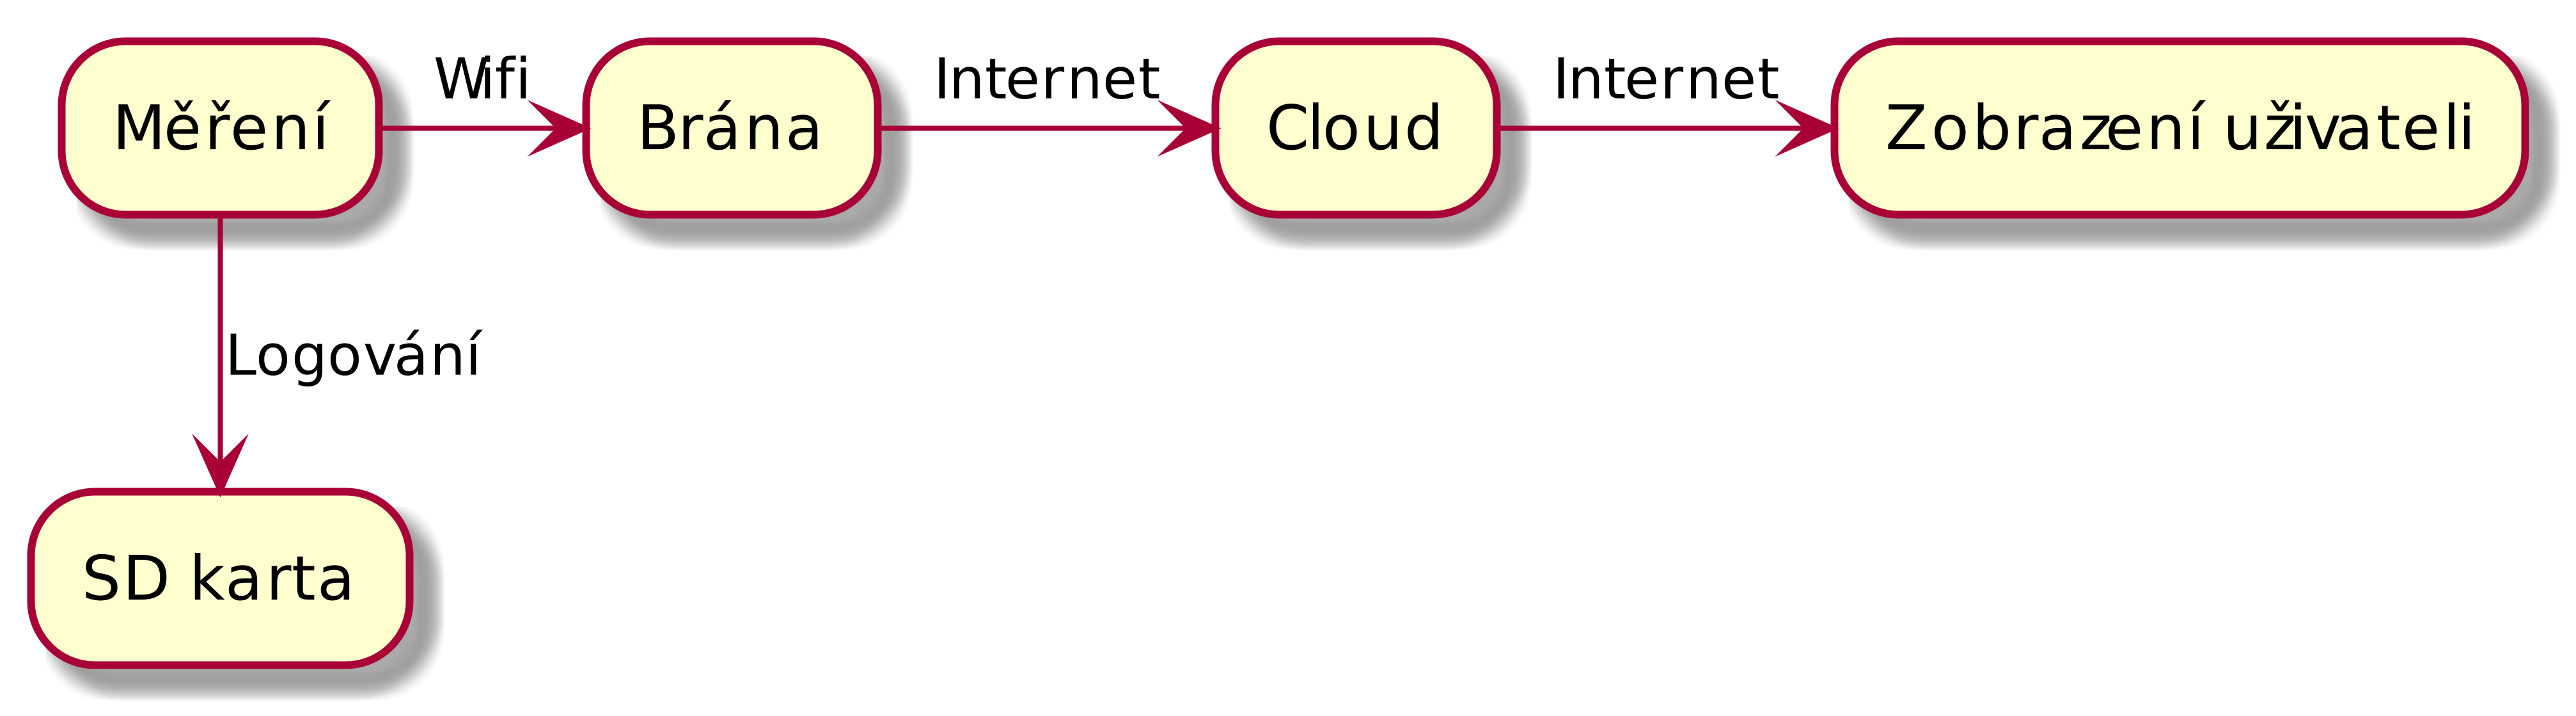
\includegraphics{dataFlow.png}
\end{figure}

% UI + analýza
Uživatelské rozhraní pro zobrazení hodnot jsem se rozhodl z důvodu co největší přenositelnosti ji implementovat jako 
webovou stránku. Takže celá jeho logika a vykreslování bude řešená v javascriptu a až na klientském zařízení, cloud 
použiji pouze na to, abych z něj vytáhl potřebná data a samozřejmě na hostování celé aplikace. Na této stránce určitě 
zobrazím graf vývoje změřených hodnot, myslím že v základu by mohlo stačit tak posledních 48 hodin, ale asi bych přidal 
možnost i delších časových úseků. Z dalších údajů bych si zobrazil tak možná medián naměřených hodnot a možná průměr, 
ale další údaje mi už přijdou zbytečné. Další analýzy dělat nebudu, spíše  bude sledovat jak se kytičkám daří a případně 
je po nasbírání zkušeností doplním.

% bezpečnost
Co se otázky bezpečnosti týče, tak vynechám šifrování na cestě od senzoru do brány, zejména z důvodu jednoduššího ladění 
a implementace, avšak co na této cestě doplním je elektronický podpis zprávy, aby se mi nikdo nefušoval do komunikace. 
Zabezpečení komunikace s cloudem už budu řešit prostředky té dané služby i co se zobrazení hodnot týče.
